\section{Мониторинг загрязнения воздуха}
\begin{frame}{\insertsectionhead}
    \begin{columns}[c]
        \begin{column}{.55\linewidth}
        \footnotesize
        Наблюдения за состоянием атмосферного воздуха на территории Саратовской области проводятся 
        Саратовским центром по гидрометеорологии и мониторингу окружающей среды
        в двух крупнейших промышленных центрах области: в г. Саратове и в г. Балаково.
        \smallskip

        Наблюдения за состоянием атмосферного воздуха городов проводятся ежедневно на 13 станционарных постах, 
        с периодичностью шесть дней в неделю, три раза в сутки.
        
        \smallskip
        Загрязнение атмосферного воздуха определяется по значениям концентраций примесей. 
        Степень загрязнения оценивается при сравнении концентраций примеси в атмосферном 
        воздухе с предельно допустимыми концентрациями (ПДК). 
        \end{column}

        \begin{column}{.42\linewidth}
            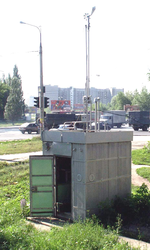
\includegraphics[width=0.7\textwidth]{assets/pnz.png}
        \end{column}
    \end{columns}
\end{frame}
